\chapter{Aplicação a dados reais}


\section{Complexo de Anitápolis}
\label{subsec:anitapolis_complex}


O complexo alcalino-carbonatítico de Anitápolis forma um corpo circular 
($\approx 6$ km$^{2}$) que contém magnetita e intrudiu leucogranitos do Cretáceo Inferior ($132$ Ma), aparentemente na mesma época do derramamento basáltico da formação Serra Geral ($133-130$ Ma) na Bacia do Paraná \citep{scheibe_etal2005, gomes_etal2018}. 
De acordo com \citet{riccomini_etal2005} e \citet{gomes_etal2018}, 
este complexo não mostra um controle estrutural claro e ainda há debate sobre sua intrusão. 
Por exemplo, \citet{melcher_coutinho1966} propôs a influência de falhas orientadas preferencialmente em N-S
enquanto que \citet{horbach_marimon1980} e \citet{scheibe_etal2005} consideram que o complexo é controlado por lineamentos N30W e Leste-Oeste, respectivamente.

As Figuras \ref{fig:anitapolis_data}a e \ref{fig:anitapolis_data}b exibem a anomalia de campo total observada e o campo regional estimado sobre o complexo de Anitápolis, respectivamente.
O levantamento aéreo foi adquirido com linhas N-S e L-O espaçadas em $500$ m e $10.000$ m umas das outras, respectivamente, sobre a superfície ondulada mostrada na Figura \ref{fig:anitapolis_data}c. 
A Figura \ref{fig:anitapolis_data}d mostra a topografia da área de estudo.
A inclinação e a declinação do campo geomagnético principal na área de estudo, para a época da aquisição $(2009-2011)$, são $-37,05^{\circ}$ e 
$-18,17^{\circ}$, respectivamente.

A Figura \ref{fig:anitapolis_rtp_residual}a mostra a anomalia de campo total residual obtida pela subtração do campo regional estimado (Fig. \ref{fig:anitapolis_data}b)
da anomalia de campo total observada (Fig. \ref{fig:anitapolis_data}a).
A partir dessa anomalia residual, foi calculada a anomalia RTP mostrada na Figura \ref{fig:anitapolis_rtp_residual}b utilizando a direção de magnetização estimada por \citet{reis_etal2019} com inclinação $-21^{\circ}$ e declinação $-11^{\circ}$.
A área positiva da anomalia RTP estimada foi usada para definir as aproximações iniciais para todas as soluções L2 (Fig. \ref{fig:anitapolis_l2_result}) e L1 
(Fig. \ref{fig:anitapolis_l1_result}) obtidas pelo método ao realizar a inversão da anomalia de campo total residual mostrada na Figura \ref{fig:anitapolis_rtp_residual}a.
Todas essas soluções L2 e L1 foram obtidas através da utilização do seguinte conjunto de pesos normalizados $\tilde{\alpha}_{\ell}$ (Equação \ref{eq:alphas}):
$\tilde{\alpha}_{1} = 10^{-4}$, $\tilde{\alpha}_{2} = 10^{-3}$, 
$\tilde{\alpha}_{3} = 10^{-4}$, $\tilde{\alpha}_{4} = 10^{-8}$, e 
$\tilde{\alpha}_{5} = 10^{-5}$.

A Figura \ref{fig:anitapolis_l2_result}a mostra os valores da função objetivo produzidos pelas 100 soluções L2 obtidas por uma malha de varredura de $10 \times 10$ valores de profundidade do topo $z_{0}$ e intensidade de magnetização total $m_{0}$.
A melhor solução L2 possui uma profundidade do topo de $z_{0} = 0$ m, intensidade de magnetização total de $m_{0} = 15$ A/m e uma profundidade da base em $3032,7$ m.
A Figura \ref{fig:anitapolis_l1_result}a exibe os valores da função objetivo produzidos pelas 100 soluções L1 obtidas por uma malha de varredura de $10 \times 10$ valores de profundidade do topo $z_{0}$ e intensidade de magnetização total $m_{0}$.
A melhor solução L1 possui uma profundidade do topo de $z_{0} = 240$ m, intensidade de magnetização total de $m_{0} = 14$ A/m e uma profundidade da base em $3259,6$ m.

As intensidades de magnetização total das soluções estão ambas em acordo com as medidas de laboratório conduzidas por \citet{valdivia_etal2009} nas amostras de rochas do complexo de Jacupiranga, outro complexo alcalino localizado ao norte da área de estudo, com a mesma idade do complexo de Anitápolis. De acordo com o esses autores,
os valores podem variar de $\approx 0,01$ a $\approx 29,90$ A/m.
A extensão vertical total da melhor solução L2 ($3032,7$ m) é muito similar à extensão da solução L1 ($3019,6$ m). 
Ambas as soluções mostram uma intrusão com direção preferencial de N30W tendo praticamente a mesma forma,
alinhada com o baixo da topografia exibida na Figura \ref{fig:anitapolis_data}d (no centro do retângulo rosa). 
Essa orientação é consistente com a proposta por \citet{horbach_marimon1980} para um grande lineamento na área de estudo.
O topo da solução L1 é mais profundo do que o da solução L2, 
o que sugere a possível presença de uma pequena fonte não-alvo rasa.
Finalmente, a Tabela \ref{tab:anitapolis} mostra que a solução L1 é superior à solução L2 mesmo que ambas exibam semelhanças em suas geometrias.

\begin{table}[h]\label{tab:anitapolis}
	\caption{Valores dos vínculos na iteração final para as melhores soluções L2 e L1 da aplicação ao complexo de Anitápolis (Eqs. \ref{eq:phi1}, \ref{eq:phi2}, \ref{eq:phi3}, \ref{eq:phi4} e \ref{eq:phi5}).}
	\centering
	\vspace{0.5cm}
	\begin{tabular}{c|ccccc}
		Vínculo & $ \varphi _1 $ & $ \varphi _2 $ &  $ \varphi _3 $ &  $ \varphi _4 $ &  $ \varphi _5 $ \\
		\hline
		Solução L2 & $ 1,48 $ & $ 22,2 $ & $ 17,24 $ & $3,00\times 10^{-3} $ & $ 0,48 $ \\ 
		Solução L1 & $ 0,12 $ & $ 1,63 $ & $ 1,77 $ & $8,30\times 10^{-4} $ & $ 0,14 $
	\end{tabular}
\end{table}

\pagebreak
\begin{figure}[!htb]
	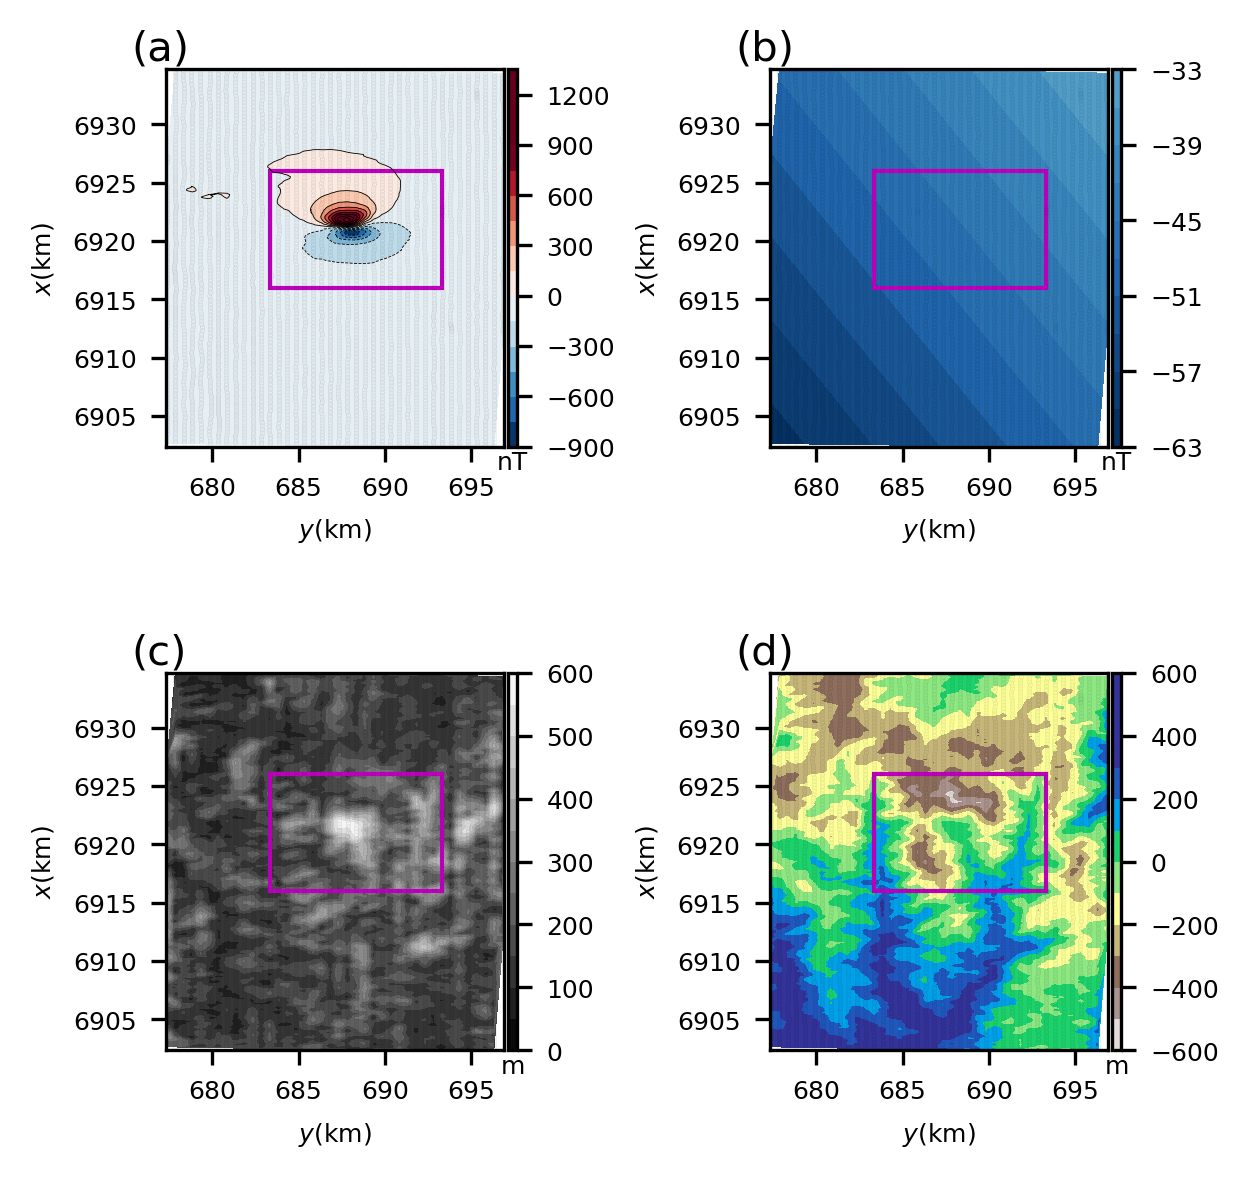
\includegraphics[width=\textwidth]{anitapolis_data.png}
	\caption{Aplicação aos dados do complexo de Anitápolis. 
		(a) Anomalia de campo total observada.
		(b) Polinômio de primeira ordem que representa o campo regional.
		(c) e (d) Altura geométrica dos pontos de observação e topografia,
		ambas referenciadas ao elipsoide WGS84. Por simplicidade, foi removida uma constante de $800$ m de seus valores. As coordenadas UTM estão referenciadas ao meridiano central $51^{\circ}$. Os pontos pretos representam os pontos observados. Apenas os dados delimitados pelo retângulo rosa foram usados para a inversão. 
	}
	\label{fig:anitapolis_data}
\end{figure}
\pagebreak
\begin{figure}[!htb]
	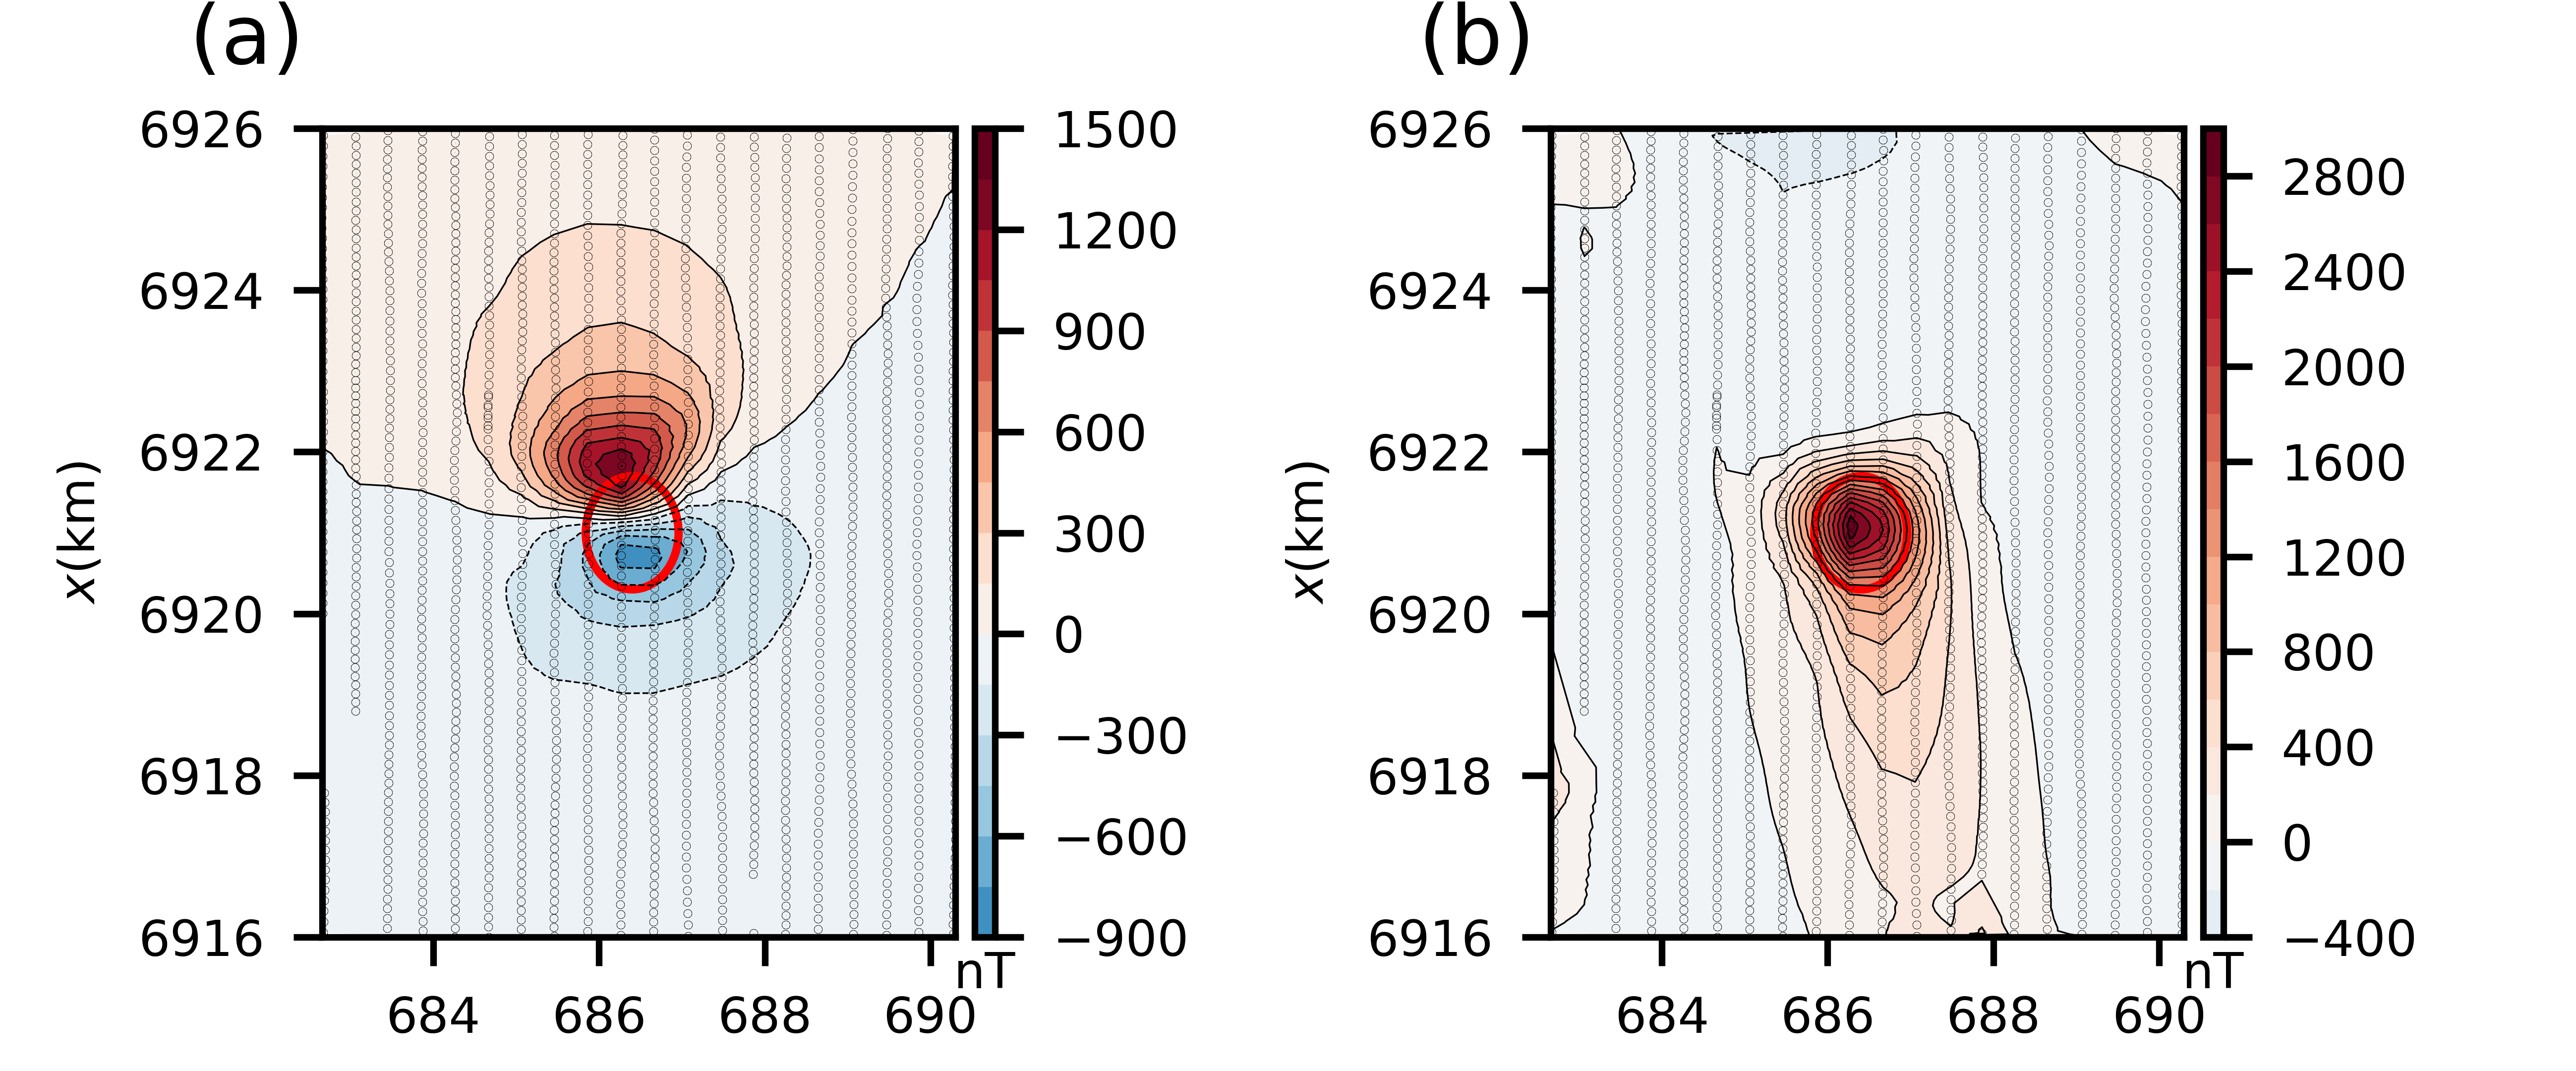
\includegraphics[width=\textwidth]{anitapolis_rtp.png}
	\caption{Aplicação aos dados do complexo de Anitápolis. 
		(a) e (b) Anomalias residual e RTP sobre a área de estudo definida pelo retângulo rosa na Figura \ref{fig:anitapolis_data}.
		A linha vermelha representa a projeção horizontal das aproximações iniciais usadas nas inversões subsequentes (prismas vermelhos nas Figuras 
		\ref{fig:anitapolis_l2_result}c e \ref{fig:anitapolis_l1_result}c).
	}
	\label{fig:anitapolis_rtp_residual}
\end{figure}

\pagebreak

\begin{figure}[!htb]
	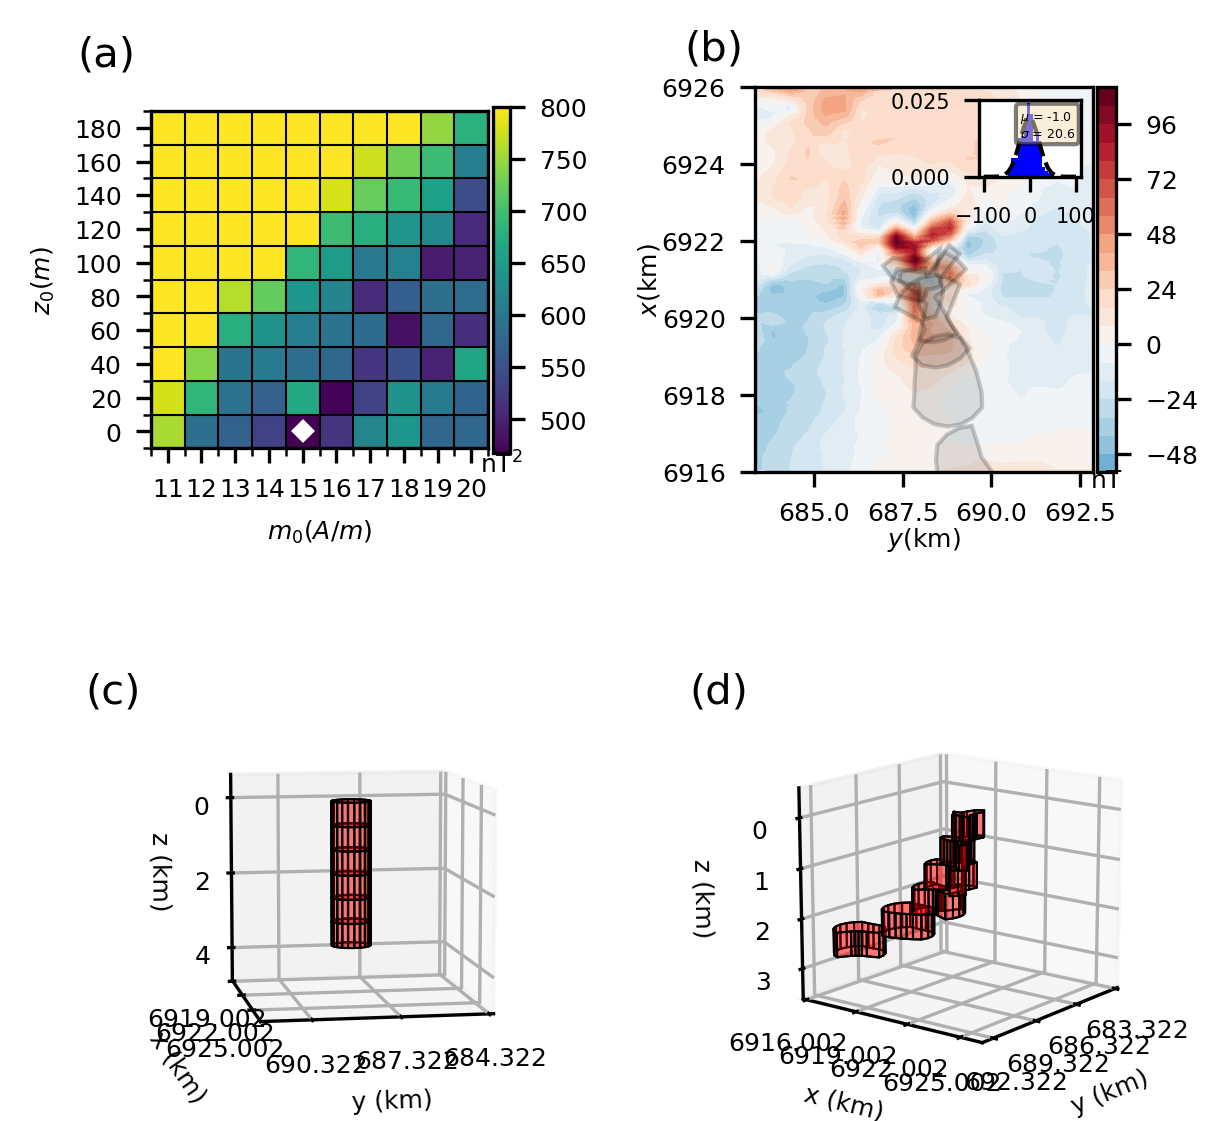
\includegraphics[width=\textwidth]{anitapolis-l2-solution.png}
	\caption{Soluções L2 obtidas para o complexo de Anitápolis. 
		(a) Mapa discreto da função objetivo produzida pelos modelos obtidos a partir da varredura de valores de profundidade do topo $z_{0}$ e intensidade de magnetização total $m_{0}$. 
		O losango branco representa os valores de $m_{0}$ e $z_{0}$ que definem a melhor solução L2.
		(b) Resíduos entre a anomalia de campo total residual (Fig. \ref{fig:anitapolis_rtp_residual}a) e os dados preditos (não exibidos) produzidos pela melhor solução L2 (prismas vermelhos no painel d). 
		O histograma dos resíduos inserido em (b) mostra a curva
		Gaussiana ajustada (linha tracejada). 
		(c) e (d) Visualizações em perspectiva da aproximação inicial e da melhor solução, respectivamente.
	}
	\label{fig:anitapolis_l2_result}
\end{figure}

\pagebreak

\begin{figure}[!htb]
	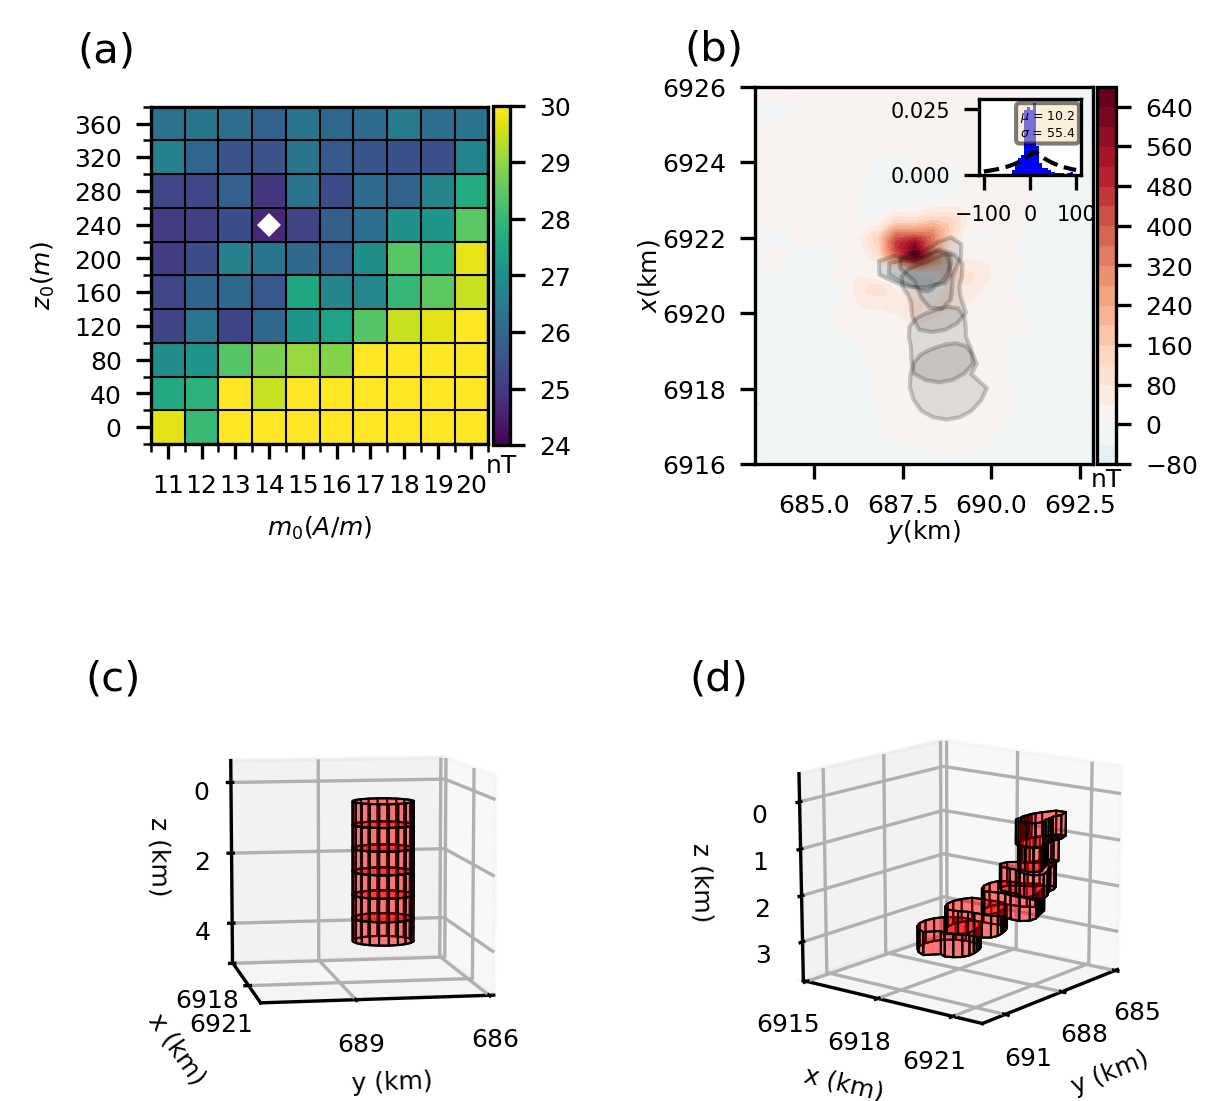
\includegraphics[width=\textwidth]{anitapolis-l1-solution.png}
	\caption{Soluções L1 obtidas para o complexo de Anitápolis. 
		(a) Mapa discreto da função objetivo produzida pelos modelos obtidos a partir da varredura de valores de profundidade do topo $z_{0}$ e intensidade de magnetização total $m_{0}$. 
		O losango branco representa os valores de $m_{0}$ e $z_{0}$ que definem a melhor solução L1.
		(b) Resíduos entre a anomalia de campo total residual (Fig. \ref{fig:anitapolis_rtp_residual}a) e os dados preditos (não exibidos) produzidos pela melhor solução L1 (prismas vermelhos no painel d). 
		O histograma dos resíduos inserido em (b) mostra a curva
		Laplaciana ajustada (linha tracejada). 
		(c) e (d) Visualizações em perspectiva da aproximação inicial e da melhor solução, respectivamente.
	}
	\label{fig:anitapolis_l1_result}
\end{figure}
\pagebreak


\section{Complexo de Diorama}
\label{subsec:diorama_complex}


A província alcalina de Goiás (PAGO) é resultado de um magmatismo máfico-alcalino que ocorreu no final do Cretáceo, na borda da Bacia do Paraná.
Ela é associada com uma grande variedade petrográfica que incluem complexos máficos e ultra-máficos, intrusões alcalinas subvulcânicas e vulcânicas que coincidem com uma bem definida tendência de falhas no embasamento de N50E \citep{junqueirabrod_etal2002, junqueira_brod2005}.
Diferentes estudos geofísicos indicam que as anomalias magnéticas associadas às intrusões alcalinas na PAGO são afetadas por notáveis magnetizações remanentes \citep[por exemplo,][]{dutra_etal2012, marangoni_mantovani2013, 
dutra_etal2014, oliveirajr_etal2015, zhang-2018, reis_etal2020}.

As Figuras \ref{fig:diorama_data}a e \ref{fig:diorama_data}b mostram, respectivamente, 
a anomalia de campo total observada e o campo regional estimado sobre o complexo de Diorama na parte norte da PAGO \citep{junqueira_brod2005,
marangoni_mantovani2013, oliveirajr_etal2015}.
O levantamento aéreo foi adquirido com linhas N-S e L-O espaçadas em $500$ m e $10.000$ m umas das outras, respectivamente, sobre a superfície ondulada mostrada na Figura 
\ref{fig:diorama_data}c. 
A Figura \ref{fig:diorama_data}d mostra a topografia na área de estudo.
A inclinação e a declinação do campo geomagnético principal na área de estudo, para a época da aquisição $(2004)$, são $-19,5^{\circ}$ e 
$-18,5^{\circ}$, respectivamente.

A Figura \ref{fig:diorama_rtp_residual}a mostra a anomalia de campo total residual obtida pela subtração do campo regional estimado (Fig. \ref{fig:diorama_data}b)
da anomalia de campo total observada (Fig. \ref{fig:diorama_data}a).
A partir dessa anomalia residual, foi calculada a anomalia RTP mostrada na Figura \ref{fig:diorama_rtp_residual}b utilizando a direção de magnetização estimada por \citet{zhang-2018} com inclinação $-46^{\circ}$ e declinação $24^{\circ}$.
Considerando o máximo e o máximo gradiente (ponto de inflexão), a área positiva da anomalia RTP estimada foi usada para definir as aproximações iniciais para todas as soluções L2 (Fig. \ref{fig:diorama_l2_result}) e L1 
(Fig. \ref{fig:diorama_l1_result}) obtidas pelo método ao realizar a inversão da anomalia de campo total residual mostrada na Figura \ref{fig:diorama_rtp_residual}a.
Todas essas soluções L2 e L1 foram obtidas através da utilização do seguinte conjunto de pesos normalizados $\tilde{\alpha}_{\ell}$ (Equação \ref{eq:alphas}):
$\tilde{\alpha}_{1} = 10^{-4}$, $\tilde{\alpha}_{2} = 10^{-4}$, 
$\tilde{\alpha}_{3} = 10^{-4}$, $\tilde{\alpha}_{4} = 10^{-6}$, e
$\tilde{\alpha}_{5} = 10^{-6}$.

A Figura \ref{fig:diorama_l2_result}a mostra os valores da função objetivo produzidos pelas 100 soluções L2 obtidas por uma malha de varredura de $10 \times 10$ valores de profundidade do topo $z_{0}$ e intensidade de magnetização total $m_{0}$.
A melhor solução L2 possui uma profundidade do topo de $z_{0} = 200$ m, intensidade de magnetização total de $m_{0} = 19$ A/m e uma profundidade da base em $2090,0$ m.
A Figura \ref{fig:diorama_l1_result}a exibe os valores da função objetivo produzidos pelas 100 soluções L2 obtidas por uma malha de varredura de $10 \times 10$ valores de profundidade do topo $z_{0}$ e intensidade de magnetização total $m_{0}$.
A melhor solução L1 possui uma profundidade do topo de $z_{0} = 250$ m, intensidade de magnetização total de $m_{0} = 18$ A/m e uma profundidade da base em $2692,0$ m.

As intensidades de magnetização total das soluções estão ambas em acordo com as medidas de laboratório conduzidas por \citet{dutra2011} e \citet{dutra_etal2014} 
em amostras de rochas da PAGO. Eles encontraram valores que variam de $\approx 0,01$ a $20$ A/m.
A extensão vertical total da melhor solução L2 ($1890,0$ m) é $\approx 500$ m 
menor que a extensão da melhor solução L1 ($2442,0$ m), o que é consistente com a intensidade de magnetização menor da solução L1.
A extensão vertical total da solução L1 ($2442,0$ m), entretanto, é significativamente menor do que a obtida por \citet[][Fig. 4.9, p. 78]{dutra2011} para o complexo de Diorama ($\approx 3000,0$ m). 
É importante enfatizar que \cite{dutra2011} obteve essa extensão vertical total indiretamente a partir da distribuição de susceptibilidade magnética estimada em uma malha 3D pouco refinada de prismas retangulares justapostos com lado de $1$ km de comprimento e valores máximos de susceptibilidade limitados a $0,01$ SI.
Essa malha foi projetada para investigar não só o complexo de Diorama como também todas as anomalias produzidas por extensos complexos alcalinos na área de estudo. Como consequência, os resultados apresentados por
\citet{dutra2011}, também relatado por \citet{marangoni_mantovani2013}, não parecem ter resolução espacial suficiente para representar o complexo de Diorama, que é relativamente menor que os complexos ao seu redor.
Essa falta de resolução espacial associada ao limite superior imposto à distribuição de susceptibilidade magnética podem resultar em uma extensão vertical total exagerada obtida para o complexo de Diorama.
Comparado à abordagem utilizada por \citet{dutra2011}, o método apresentado neste trabalho é capaz de representar o complexo de Diorama com uma maior resolução espacial e esta pode ser a principal causa da estimativa discrepante da extensão vertical total.

A solução L2 mostra uma forma complexa que depende da profundidade com nenhum controle estrutural aparente. É possível notar que seu prisma mais profundo possui uma área maior que a dos prismas restantes. As características dessa solução assemelham-se às da solução L2 obtida para o dado sintético com a presença de uma fonte não-alvo pequena (Fig. \ref{fig:small_l2_result}).
Por outro lado, a Figura \ref{fig:diorama_l1_result} mostra uma solução L1 com uma forma que varia continuamente ao longo da profundidade que parece ser influenciada por uma falha aproximadamente orientada a N50E. Essa direção concorda com a relatada por
\citet{junqueirabrod_etal2002} para dique que cruzam o embasamento Pré-cambriano na área de estudo.
Esses resultados sugerem a presença de fontes não-alvo rasas localizadas próximas ao topo do complexo de Diorama.
Segundo a Tabela \ref{tab:diorama}, a solução L1 é significativamente superior à solução L2, incorporando melhor a informação a priori introduzida.

\begin{table}[h]\label{tab:diorama}
	\caption{Valores dos vínculos na iteração final para as melhores soluções L2 e L1 da aplicação ao complexo de Diorama (Eqs. \ref{eq:phi1}, \ref{eq:phi2}, \ref{eq:phi3}, \ref{eq:phi4} e \ref{eq:phi5}).}
	\centering
	\vspace{0.5cm}
	\begin{tabular}{c|ccccc}
		Vínculo & $ \varphi _1 $ & $ \varphi _2 $ &  $ \varphi _3 $ &  $ \varphi _4 $ &  $ \varphi _5 $ \\
		\hline
		Solução L2 & $ 29,24 $ & $ 64,05 $ & $ 1,37 $ & $ 4,24 $ & $ 0,19 $ \\ 
		Solução L1 & $ 7,57 $ & $ 6,61 $ & $ 0,35 $ & $ 2,42 $ & $ 0,22 $
	\end{tabular}
\end{table}


%% Application to Diorama data

\begin{figure}[!htb]
	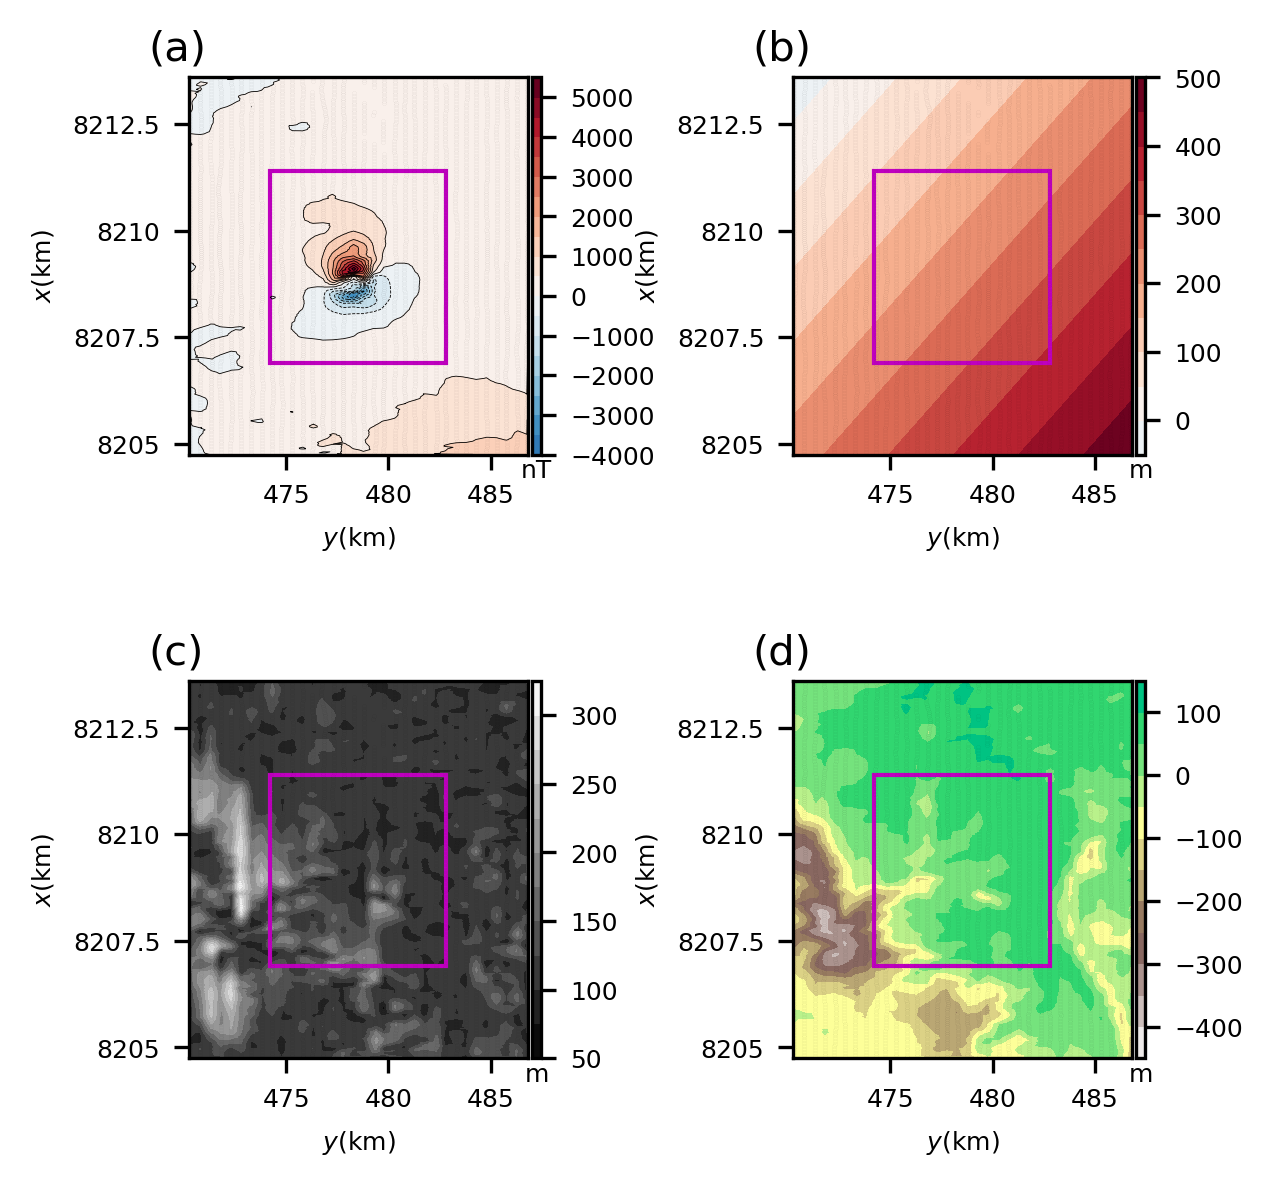
\includegraphics[width=\textwidth]{diorama_data.png}
	\caption{Aplicação aos dados do complexo de Diorama. 
		(a) Anomalia de campo total observada.
		(b) Polinômio de primeira ordem que representa o campo regional.
		(c) e (d) Altura geométrica dos pontos de observação e topografia,
		ambas referenciadas ao elipsoide WGS84. Por simplicidade, foi removida uma constante de $430$ m de seus valores. As coordenadas UTM estão referenciadas ao meridiano central $51^{\circ}$. Os pontos pretos representam os pontos observados. Apenas os dados delimitados pelo retângulo rosa foram usados para a inversão. 
	}
	\label{fig:diorama_data}
\end{figure}
\pagebreak

\begin{figure}[!htb]
	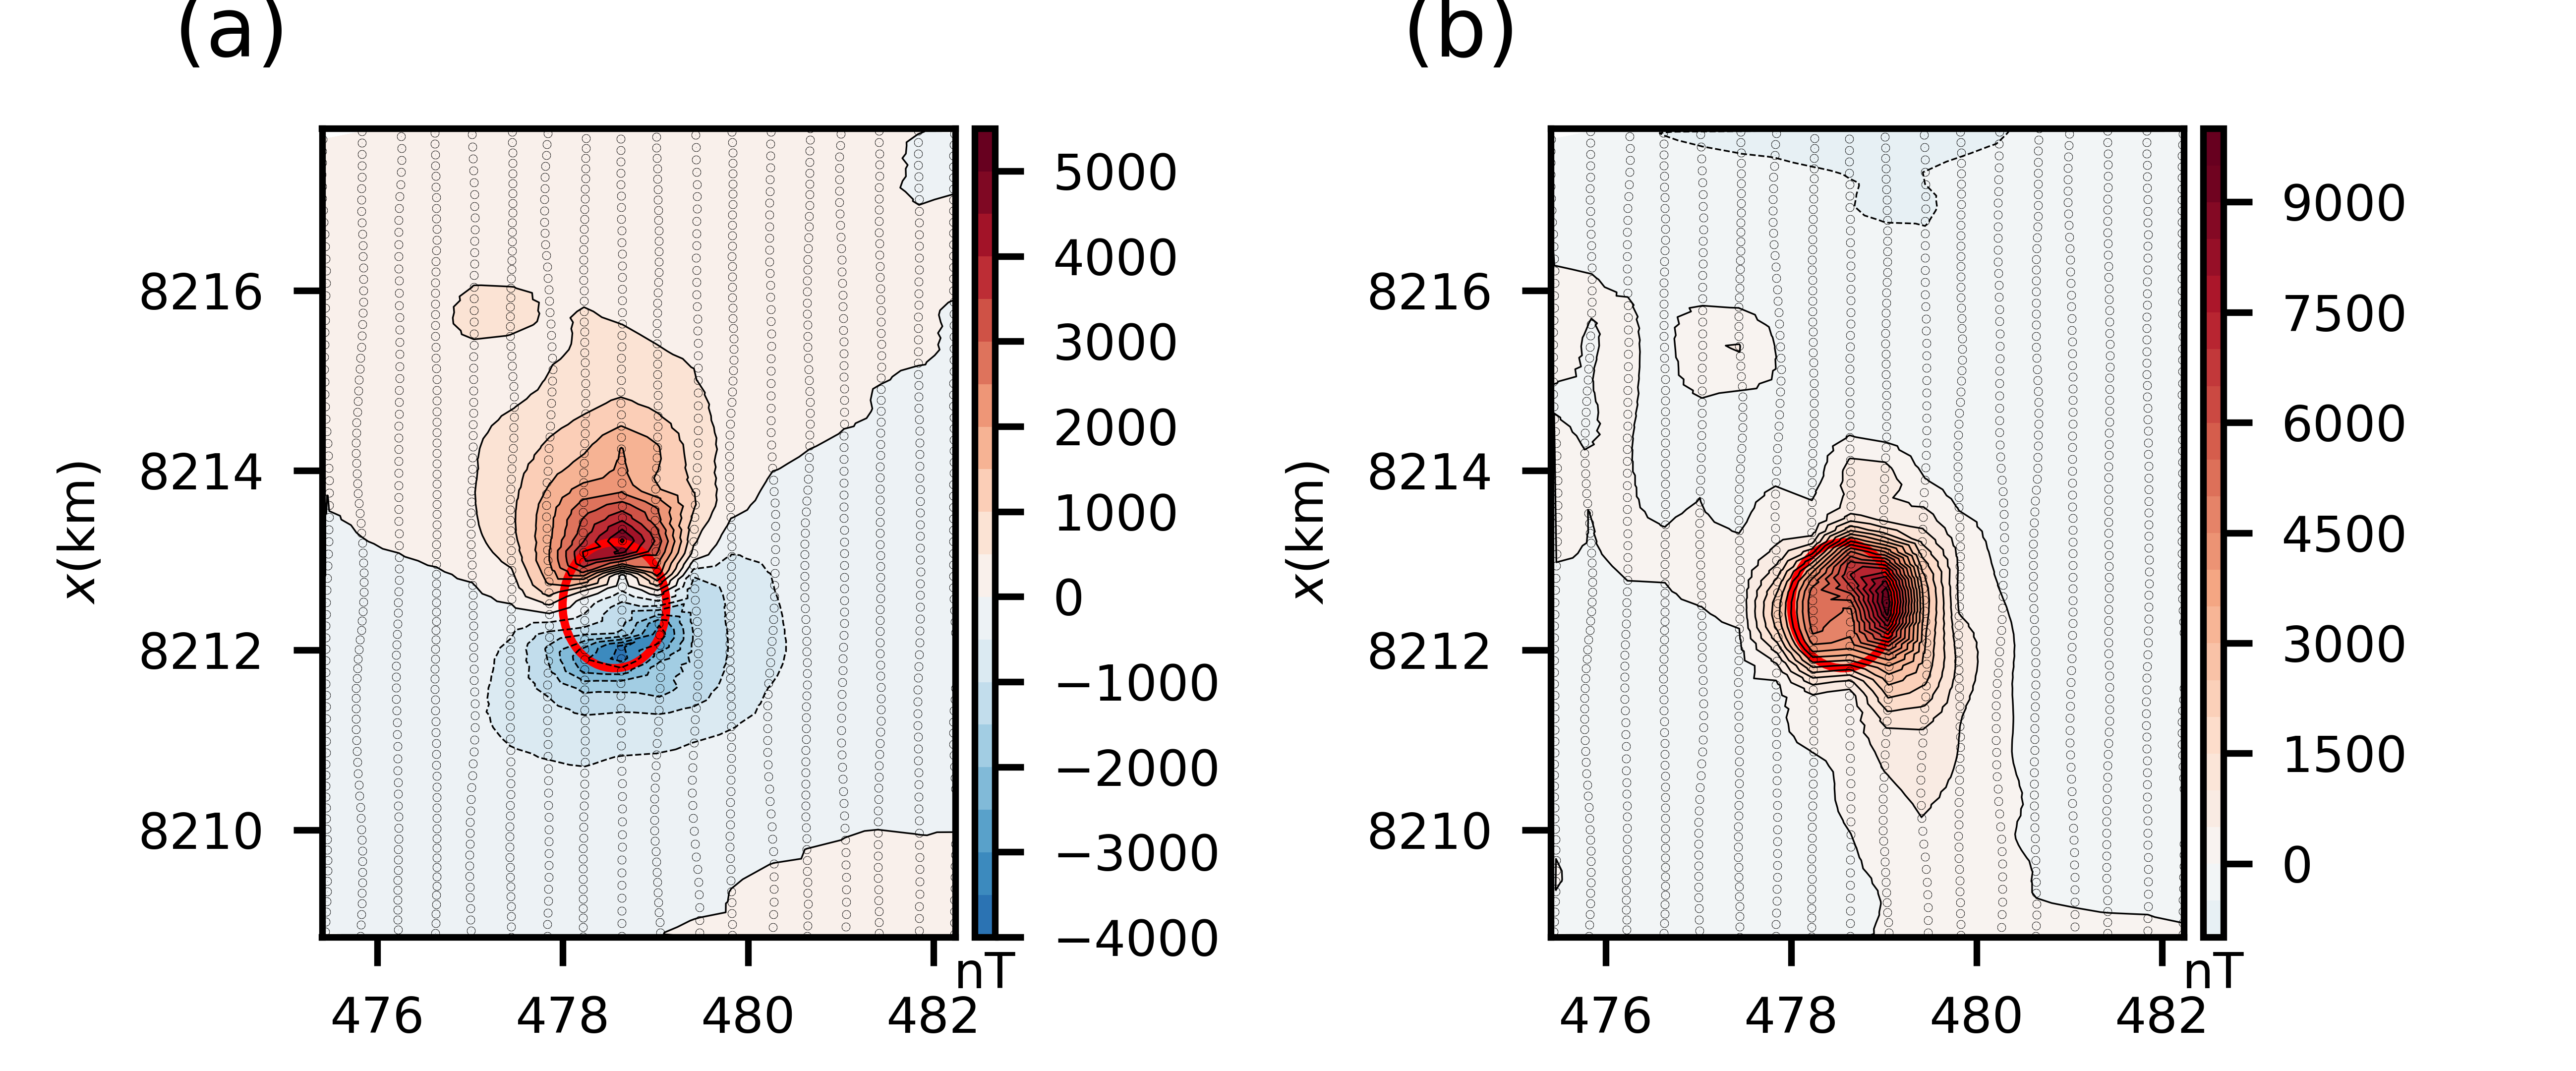
\includegraphics[width=\textwidth]{diorama_rtp.png}
	\caption{Aplicação aos dados do complexo de Diorama. 
		(a) e (b) Anomalias residual e RTP sobre a área de estudo definida pelo retângulo rosa na Figura \ref{fig:diorama_data}.
		A linha vermelha representa a projeção horizontal das aproximações iniciais usadas nas inversões subsequentes (prismas vermelhos nas Figuras \ref{fig:diorama_l2_result}c e \ref{fig:diorama_l1_result}c).
	}
	\label{fig:diorama_rtp_residual}
\end{figure}

\pagebreak
\begin{figure}[!htb]
	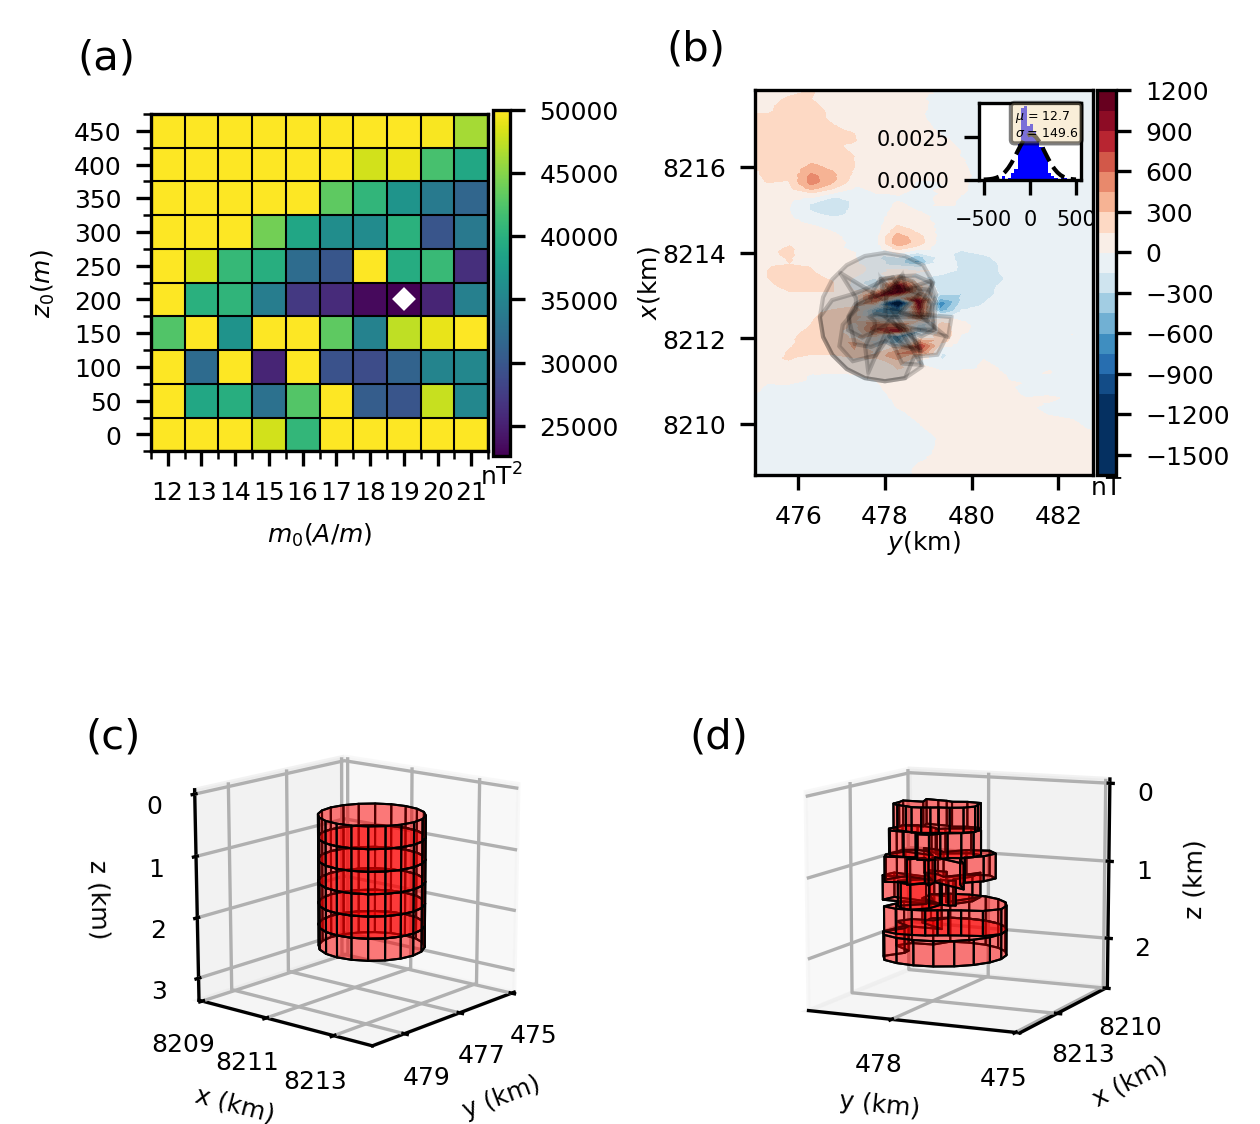
\includegraphics[width=\textwidth]{diorama-l2-solution.png}
	\caption{Soluções L2 obtidas para o complexo de Diorama. 
		(a) Mapa discreto da função objetivo produzida pelos modelos obtidos a partir da varredura de valores de profundidade do topo $z_{0}$ e intensidade de magnetização total $m_{0}$. 
		O losango branco representa os valores de $m_{0}$ e $z_{0}$ que definem a melhor solução L2.
		(b) Resíduos entre a anomalia de campo total residual (Fig. \ref{fig:diorama_rtp_residual}a) e os dados preditos (não exibidos) produzidos pela melhor solução L2 (prismas vermelhos no painel d). 
		O histograma dos resíduos inserido em (b) mostra a curva
		Gaussiana ajustada (linha tracejada). 
		(c) e (d) Visualizações em perspectiva da aproximação inicial e da melhor solução, respectivamente.
	}
	\label{fig:diorama_l2_result}
\end{figure}

\pagebreak
\begin{figure}[!htb]
	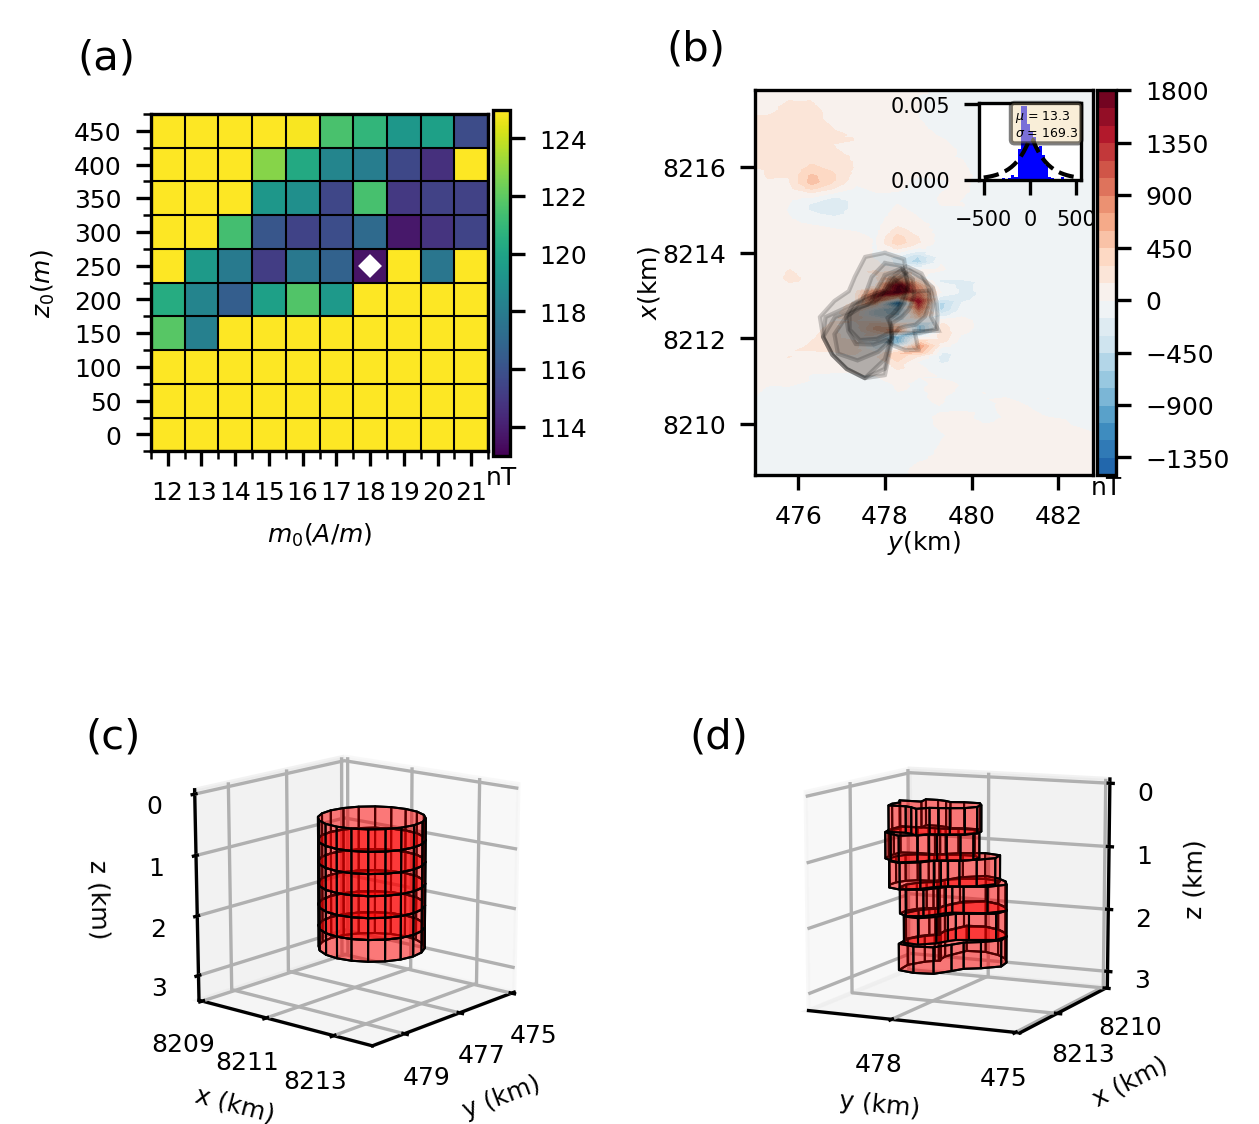
\includegraphics[width=\textwidth]{diorama-l1-solution.png}
	\caption{Soluções L1 obtidas para o complexo de Diorama. 
		(a) Mapa discreto da função objetivo produzida pelos modelos obtidos a partir da varredura de valores de profundidade do topo $z_{0}$ e intensidade de magnetização total $m_{0}$. 
		O losango branco representa os valores de $m_{0}$ e $z_{0}$ que definem a melhor solução L1.
		(b) Resíduos entre a anomalia de campo total residual (Fig. \ref{fig:diorama_rtp_residual}a) e os dados preditos (não exibidos) produzidos pela melhor solução L1 (prismas vermelhos no painel d). 
		O histograma dos resíduos inserido em (b) mostra a curva
		Laplaciana ajustada (linha tracejada). 
		(c) e (d) Visualizações em perspectiva da aproximação inicial e da melhor solução, respectivamente.
	}
	\label{fig:diorama_l1_result}
\end{figure}